% staggered_grid.tex -- fig:staggered-grid of the manuscript (App. "Consistent difference
% operators", app:lyapunov-operators). Adapted from dean.tex fig:staggered-grid.
% Build with ./run.sh, which writes staggered_grid.pdf here and copies it to
% manuscript/figures/. The figure is included at its natural size, so \footnotesize here
% matches the caption font of the two-column manuscript.
%
% (a) the central difference D applied twice reaches two nodes away and skips the two
%     neighbours (open circles): (D^2 u)_3 = (u_5 - 2u_3 + u_1)/4dx^2, the wide Laplacian.
% (b) staggered grid: G takes two nodes to the face between them, -G^T takes two faces
%     back to the node between them; -G^T G is the compact Laplacian L.
\documentclass[tikz,border=2pt]{standalone}
\usepackage{amsmath}
\begin{document}
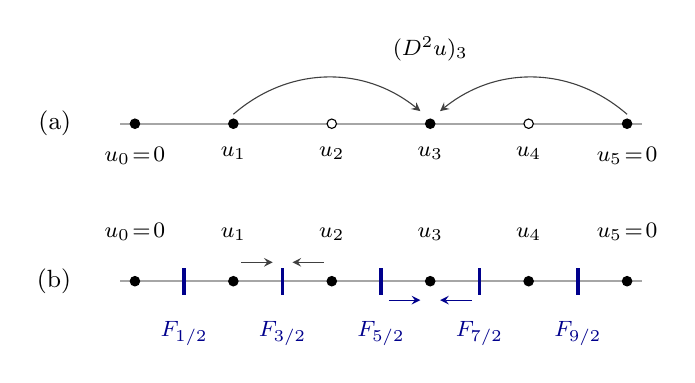
\begin{tikzpicture}[x=1.25cm, y=1cm, >=stealth, font=\footnotesize]
  % ---------------- (a) collocated grid, D applied twice ----------------
  \begin{scope}[yshift=2.0cm]
    \node[anchor=east, font=\small] at (-0.55,0) {(a)};
    \draw[gray!70, thick] (-0.15,0) -- (5.15,0);
    \foreach \i in {0,1,3,5}
      \filldraw[black] (\i,0) circle (1.7pt);
    \foreach \i in {2,4}
      \draw[black, fill=white] (\i,0) circle (1.7pt);
    \foreach \i/\lab in {0/{u_0\!=\!0}, 1/{u_1}, 2/{u_2}, 3/{u_3}, 4/{u_4}, 5/{u_5\!=\!0}}
      \node[below=5pt] at (\i,0) {$\lab$};
    \draw[->, gray!50!black] (1,0.12) to[bend left=40] (2.9,0.16);
    \draw[->, gray!50!black] (5,0.12) to[bend right=40] (3.1,0.16);
    \node at (3,0.95) {$(D^2u)_3$};
  \end{scope}
  % ---------------- (b) staggered grid: nodes and faces ----------------
  \node[anchor=east, font=\small] at (-0.55,0) {(b)};
  \draw[gray!70, thick] (-0.15,0) -- (5.15,0);
  \foreach \i in {0,1,2,3,4,5}
    \filldraw[black] (\i,0) circle (1.7pt);
  \foreach \i/\lab in {0/{u_0\!=\!0}, 1/{u_1}, 2/{u_2}, 3/{u_3}, 4/{u_4}, 5/{u_5\!=\!0}}
    \node[above=11pt] at (\i,0) {$\lab$};
  \foreach \i in {0.5,1.5,2.5,3.5,4.5}
    \draw[blue!55!black, very thick] (\i,-0.17) -- (\i,0.17);
  \foreach \i/\lab in {0.5/{F_{1/2}}, 1.5/{F_{3/2}}, 2.5/{F_{5/2}}, 3.5/{F_{7/2}}, 4.5/{F_{9/2}}}
    \node[below=11pt, blue!55!black] at (\i,0) {$\lab$};
  % G: two nodes -> the face between them
  \draw[->, gray!50!black] (1.08,0.24) -- (1.40,0.24);
  \draw[->, gray!50!black] (1.92,0.24) -- (1.60,0.24);
  % -G^T: two faces -> the node between them
  \draw[->, blue!55!black] (2.58,-0.24) -- (2.90,-0.24);
  \draw[->, blue!55!black] (3.42,-0.24) -- (3.10,-0.24);
\end{tikzpicture}
\end{document}
